\documentclass[12pt]{article}
\usepackage[margin=1in]{geometry}
\usepackage{graphicx}
\usepackage{hyperref}
\usepackage{enumitem}
\usepackage{xcolor}
\usepackage{array}
\usepackage{longtable}
\usepackage{booktabs}
\usepackage{fontspec}
\setmainfont{Roboto}
\title{Defence Submission – Hemraj Case}
\author{Legal Luminaire – Defence Team}
\date{\today}

\begin{document}
\maketitle

\section*{Overview}
The FSL report examined three distinct materials – external wall plaster (Packet A), stone‑masonry joint mortar (Packet B), and foundation concrete (Packet C). Each material is governed by different Indian Standards, faces unique scientific challenges, and requires separate procedural defence.

\section*{Plaster – Packet A}
\subsection*{Claimed Result}
\begin{itemize}[nosep]
  \item \textbf{FSL claimed ratio:} 1 : 18
  \item \textbf{Typical specification:} IS 1661:1972 (CM 1:4) – CM 1:6
\end{itemize}

\subsection*{Procedural Grounds (Critical)}
\begin{enumerate}
  \item Samples not collected in presence of contractor’s authorised representative.
  \item Storm‑weather collection – rainwater contamination.
  \item Lack of chain‑of‑custody documentation.
  \item No record of sampling date/time.
  \item No control sample provided.
  \item Insufficient sample quantity for repeat testing.
  \item Absence of proper lab‑witness.
  \item No retention of referee sample.
  \item Failure to disclose testing methodology.
\end{enumerate}

\subsection*{Technical Challenges (Material‑Specific)}
\begin{itemize}
  \item Carbonation of hardened plaster alters soluble silica.
  \item Sampling depth may have included underlying substrate.
\end{itemize}

\subsection*{Conclusion}
The 1 : 18 ratio is vitiated by all procedural violations and the two scientific factors above. The standing boundary wall demonstrates that plaster cannot be this lean. No adverse finding can be sustained.

\section*{Mortar – Packet B}
\subsection*{Claimed Result}
\begin{itemize}[nosep]
  \item \textbf{FSL claimed ratio:} 1 : 17
  \item \textbf{Typical specification:} IS 2250:1981 – M 3/M 4 (1 : 5 or 1 : 6)
\end{itemize}

\subsection*{Procedural Grounds (Critical)}
(identical to Plaster – nine items listed above)

\subsection*{Technical Challenges}
\begin{itemize}
  \item Stone‑silica contamination inevitable when hammering wet stone‑masonry.
\end{itemize}

\subsection*{Conclusion}
The 1 : 17 ratio is unreliable due to procedural violations and unavoidable stone contamination. The wall’s existence proves the mortar cannot be this lean.

\section*{Concrete – Packet C}
\subsection*{Claimed Result}
\begin{itemize}[nosep]
  \item \textbf{FSL claimed ratio:} 1 : 5.75 : 9.5 (Cement : Sand : Grit)
  \item \textbf{Typical specification:} IS 456:2000 – M10/M15 concrete.
\end{itemize}

\subsection*{Procedural Grounds (Critical)}
(identical to Plaster – nine items listed above)

\subsection*{Technical Challenges}
\begin{itemize}
  \item Chemical analysis method (IS 4031 Part 5) is not prescribed for concrete mix verification.
  \item Coarse‑aggregate silica confounds the three‑component calculation.
\end{itemize}

\subsection*{Conclusion}
Both procedural and methodological flaws invalidate the reported ratio. Proper verification requires core‑drilling (IS 516 Part 5) or petrography (ASTM C856).

\section*{Prayer}
The FSL results for all three packets be excluded from consideration or accorded no probative weight. A fresh test using the correct standard methods, with the contractor’s representative present, should be directed.

\begin{figure}[h!]
  \centering
  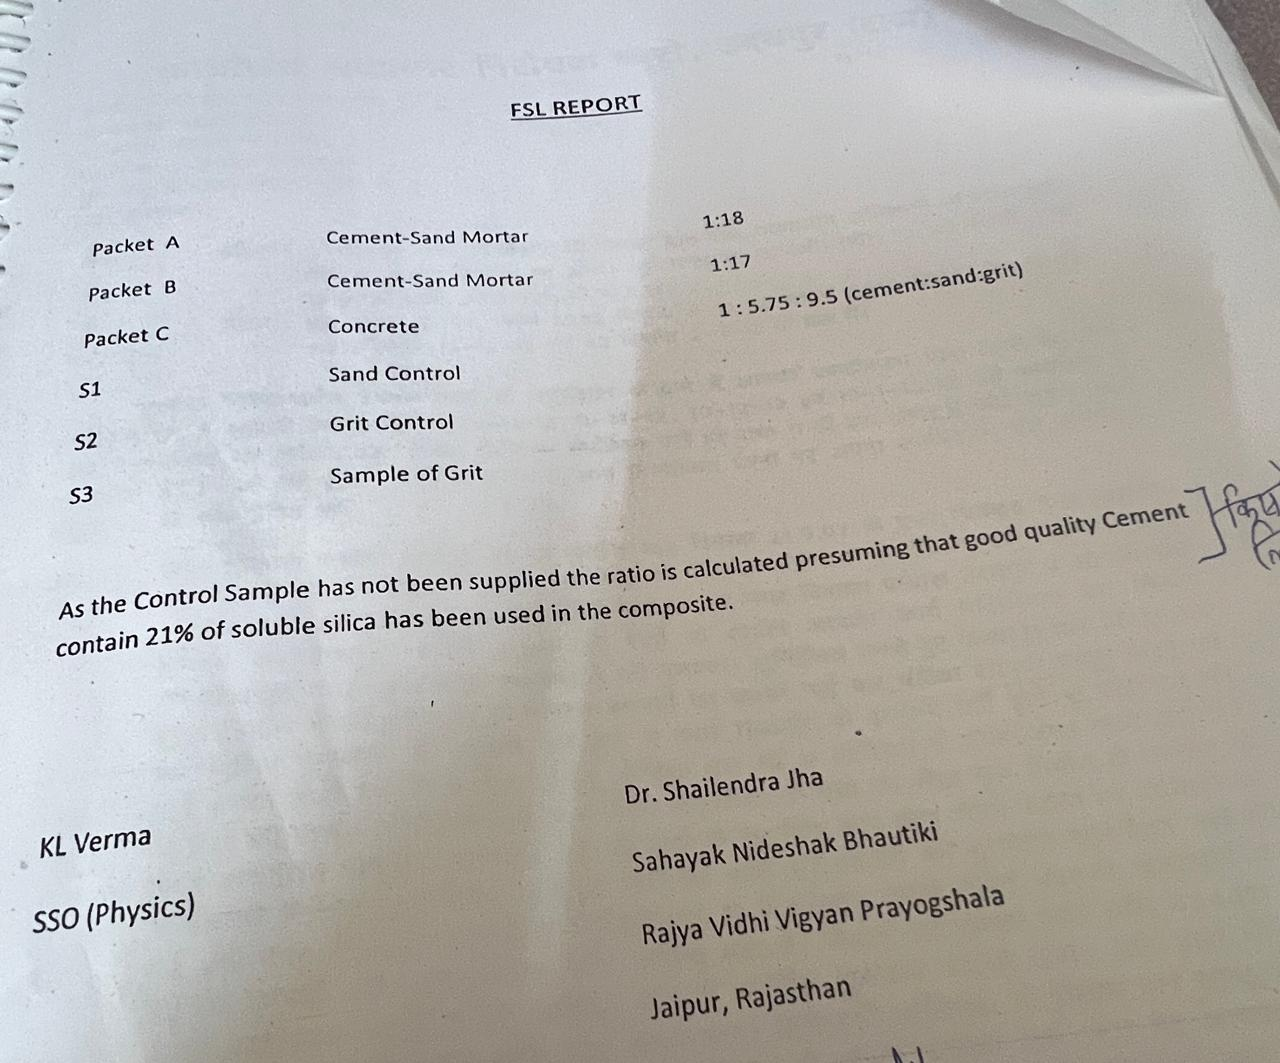
\includegraphics[width=0.8\textwidth]{FSL_TEST_REPORT_HEMRAJ_CASE_1778738761265.jpeg}
  \caption{Excerpt from the FSL report (placeholder image)}
\end{figure}

\end{document}
